\documentclass{article}
\usepackage{algorithmicx}
\usepackage{algpseudocode}
\usepackage{graphicx}
\usepackage{color}
\usepackage[utf8]{inputenc}

\begin{document}
{\noindent \Huge Problema a resolver:}
\newline \newline  El problema esta dado por la siguiente situaci\'on: 
tenemos en un $"$lista$"$ con una cantidad \textit{3$*$n} de n\'umeros(n un n\'umero fijo).\newline
Para \textit{i} desde \textit{0} a \textit{n-1}, vamos a decir la posici\'on \textit{i} en la lista va a ser \textit{Izq} del edificio \textit{i-\'esimo}, \textit{i+1} va a ser \textit{Alt} del edificio \textit{i-\'esimo} e \textit{i+2} va a ser \textit{Der} del edificio i-\'esimo.\newline
A grandes rasgos vamos a tener una lista de \textit{n} edificios (interpretamos a un edificio como una tupla \textit{$<$Izq,Alt,Der$>$}) con una base en com\'un impl\'icita que es 0.\newline
Por ejemplo para un entrada de la forma: \newline
\textit{n=3} y \textit{lista$=$ $<$1,2,3$>$,$<$4,2,7$>$,$<$2,4,6$>$} proyectada en un gr\'afico quedar\'ia:
\vspace{0.4cm}
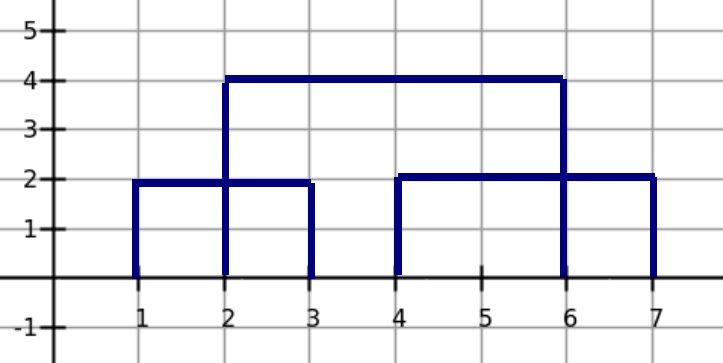
\includegraphics[width=\textwidth,height=\textheight,keepaspectratio
]{edificiosGraf1.png}
\begin {flushleft}
\end{flushleft}

Lo que queremos hacer es $"$eliminar todas las lineas interiores del gr\'afico$"$, quedarnos con su contorno se obtiene el mismo resultado  "siguiendo con el dedo el gr\'afico". \newpage
Para una \textit{lista$=$ $<$0,3,8$>$,$<$1,6,5$>$,$<$2,6,4$>$,$<$4,2,7$>$,$<$9,6,10$>$} con \textit{n=5} \newline
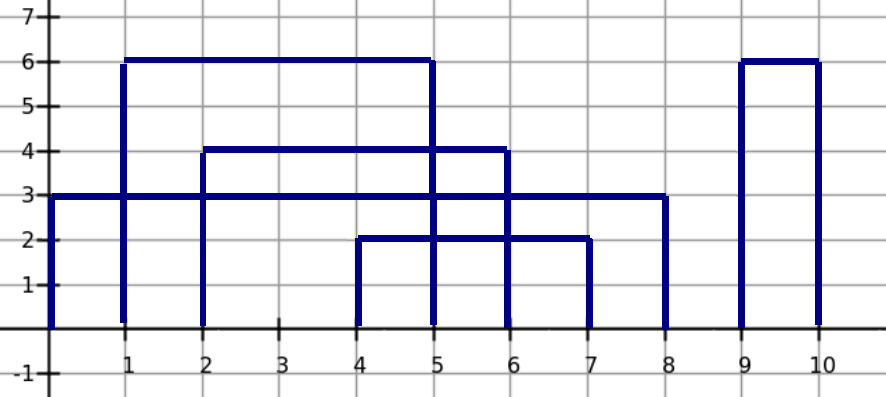
\includegraphics[width=\textwidth,height=\textheight,keepaspectratio
]{edificiosGraf2.png}
\begin {flushleft}
\end{flushleft}
el gr\'afico de eliminar las lineas interiores es:\newline
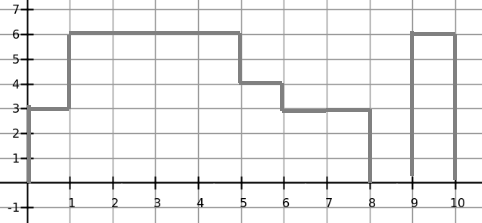
\includegraphics[width=\textwidth,height=\textheight,keepaspectratio
]{edificiosGraf2b.png}
\begin {flushleft}
\end{flushleft}
\newpage
El gr\'afico de "seguir con el dedo" es: \newline
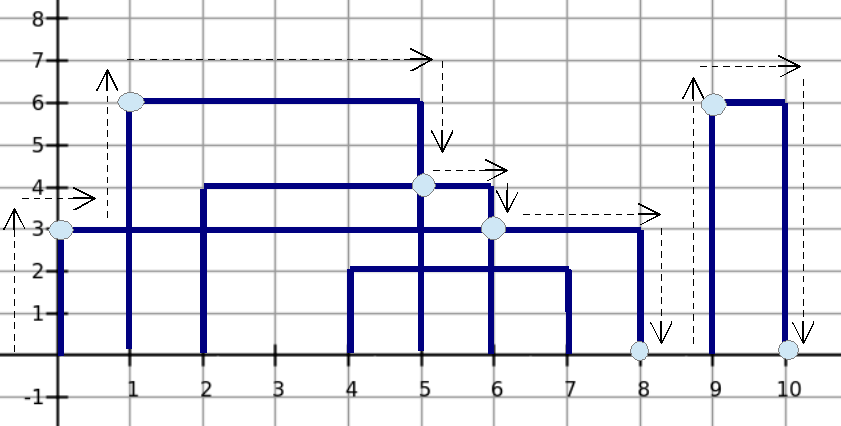
\includegraphics[width=\textwidth,height=\textheight,keepaspectratio
]{edificiosGraf2c.png}
\begin {flushleft}
\end{flushleft}

Lo que hago cuando "sigo con el dedo" es: \newline
Empezar con el primer edificio y seguimos el trazo, si me interseco con otro edificio seguir el trazo del edificio con el que me intersequ\'e desde ese punto. \newline
Si no me interseco con nadie pero hay m\'as edificios adelante "siguir con el dedo" los otros. Si no hay m\a's edificios termin\'e.\newline
Luego de ese contorno voy a obtener la soluci\'on final que son los puntos donde hay cambios($\uparrow$ $\longrightarrow$ y $\downarrow$ $\longrightarrow$). \newline

\newpage
Sea lista: lista($<$Izq,Alt,Der$>$) y n la cantidad de tuplas en la lista.

{\noindent \Huge Resoluci\'on:}
\newline \newline

\vspace{0.4cm}
\begin{algorithmic}[1]
\Procedure{ResolverEdificios}{$lista$,$n$}
	\State $comparo\gets lista[0]$
	\State $heap\gets vacio$
	\State $\textit{imprimo el primer punto}$
	\For{$(i\gets 1, n-1)$} \textit{$//$voy recorriendo los edificios}
		\State $siguiente\gets lista[i]$
		\If{$(\textit{se intersecan comparo y siguiente\color{red}{*0}})$}
			\If{$\textit{siguiente $>$ comparo en altura \color{red}{*1}}$}
				\State $\textit{imprimir solución}$
				\If{$(\textit{el heap no está vacio})$}
					\State $\textit{heap.encolar(comparo)}$
				\Else
					\If{$(\textit{comparo no está en el tope del heap}$)}
					\State$\textit{heap.encolar(comparo)}$						\EndIf			
				\EndIf
					\State $comparo\gets siguiente$
			\EndIf
			\If{$\textit{siguiente $==$ comparo en altura \color{red}{*2}}$}
				\State $\textit{imprimir solución}$
				\If{$(\textit{el heap no está vacio})$}
					\State $\textit{heap.encolar(comparo)}$
				\Else
					\If{$(\textit{comparo no está en el tope del heap}$)}
					\State$\textit{heap.encolar(comparo)}$						\EndIf			
				\EndIf
			\EndIf
			\If{$\textit{siguiente $<$ comparo en altura \color{red}{*3}}$}
				\State $heap.encolar(comparo)$
			\EndIf
			
		\EndIf \textit{(no se intersecan comparo y siguiente\color{red}{*4})}
		\If{$\textit{el heap no está vacio}$}
			\While{$\textit{heap no vacio}$}
				\If{$\textit{primero.heap termina antes que siguiente \color{red}{*5}}$}		
				\State $\textit{desencolar.heap}$
				\Else \textit{(primero.heap termina despues que siguiente \color{red}{*6})}
				\State $\textit{imprimir interseccion entre comparo y primero.heap}$
				\EndIf
			\EndWhile
		\Else{\textit{ //no pasé a nadie que cortaría a comparo, y si no corta a comparo tampoco a siguiente, como no se intersecan imprimo ambos puntos}}
		\State $\textit{imprimir comparo.Der y 0 }$
		\State $\textit{imprimir siguiente.Izq y siguiente.Alt}$
		\State $comparo\gets siguiente$
		\EndIf
	\EndFor{\textit{(no hay siguiente,puede que hayan quedado cosas en el heap \color{red}{*7}})}
	\textit{//uso a comparo que es el último edificio con el que haya en el heap}
	\While{$\textit{el heap no sea vacio}$}
	\If{$\textit{comparo termina antes que primero.heap \color{red}{*8}}$}
		\State $\textit{imprimir intersección comparo y primero.heap}$
		\State $comparo\gets heap.primero$
	\Else{\textit{(comparo termina después que el primero.heap \color{red}{*9})}}
	\State $\textit{desencolar.heap}$
	\EndIf
	\EndWhile{(\textit{ultimo punto no lo imprimo nunca\color{red}{*9})}}\newline
	\textit{$//$lo imprimo acá}
	\State $\textit{imprimir ultimo punto}$
\EndProcedure
\end{algorithmic}


\end{document}